\section{Systemarchitektur}

Bei der Aufteilung der Klassen stand die Idee der \textit{seperation of concerns} im Vordergrund. In der Implementierung spiegelt sich also der Versuch wider, durch die Struktur möglichst deutliche, voneinander unabhängige und damit leichter austauschbare Schichten zu erzeugen.

\begin{figure}[h]
	\centering
	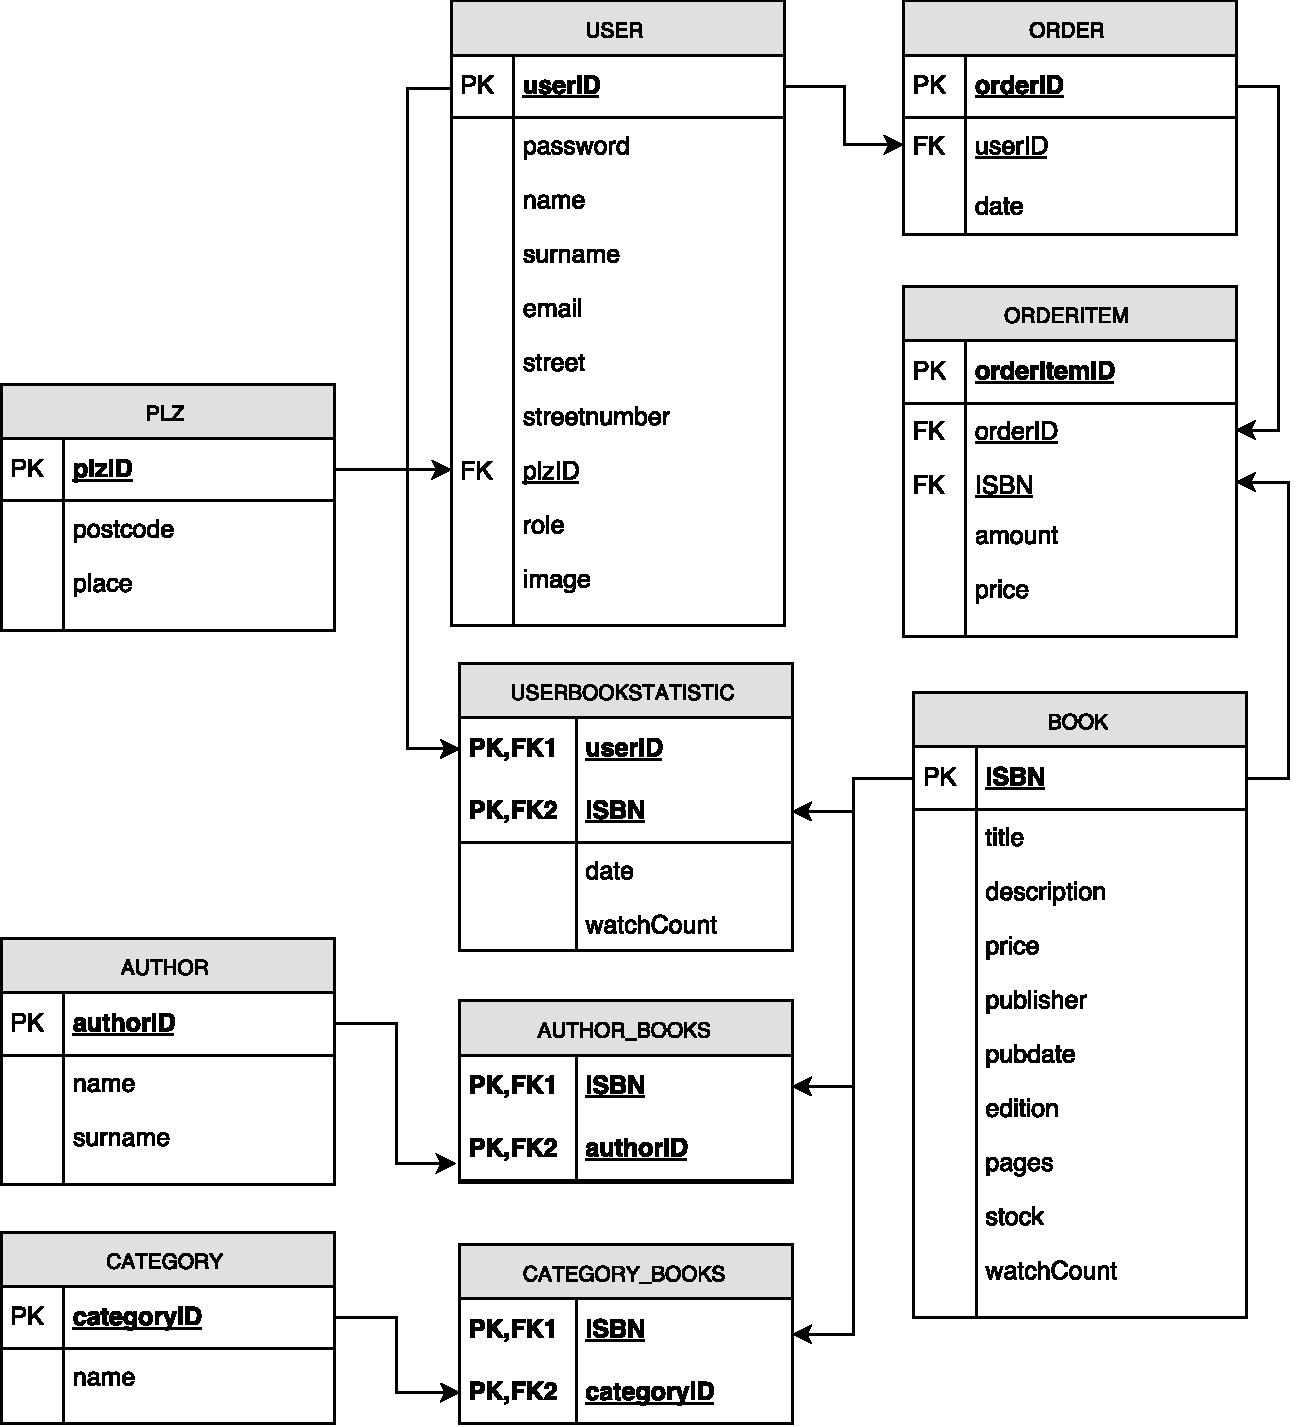
\includegraphics[width=\linewidth]{files/db-schema}
	\caption{Die Packagestruktur von \textit{kirjanystaevaet}}
	\label{fig:packages}
\end{figure}

Das System ist dabei in Anwendung (\lstinline|appl|) und Web (\lstinline|web|) unterteilt. Damit soll die klare Trennung von Programmlogik und Userinterface hervorgehoben werden. Datenbankbezogene Packages befinden sich ebenfalls im Anwendungsteil, könnten aber auch als eigenes Package ausgelagert werden. Aufgrund der engen Verbindung von Anwendung zur Datenbank (und umgekehrt) ist dies jedoch nebensächlich. Extra stehen die Konfigurationsklassen sowie eigene Exceptions.

Im Anwendungspackage herrscht eine vorwiegende Zweiteilung zwischen datenbankbezogenen (data) und datenverarbeitenden (logic) Klassen. Zusätzlich existiert ein Adminpackage, das für erste Initialisierungen des Programms zuständig ist. Data ist -- wie bei Hibernateanwendungen üblich -- in ein Package mit Entities (items) und den transaktionalen Zugriffsklassen (DAO) unterteilt. Hilfsklassen zum Aufbau von Entityobjekten sind im Builderpackage zu finden. Logic wiederrum enthält die ebenfalls konventionellen Serviceklassen, die den Zugriff auf DAOs verwalten, sowie ein Securitypackage, das die Implementation von Spring-Klassen für Login etc. enthält. Durch diese Aufteilung des Appl-Packages soll der Zugriff auf DAO-Klassen reglementiert und außerhalb der Services unnötig gemacht werden.

% Missing: Webpackage
Das Package \lstinline|web.controllers| stellt die Schnittstelle zwischen den Nutzer*innen und der Anwendungslogik dar. Auf oberster Ebene liegen neben allen Interfaces Beans für die Fehlerbehandlung sowie für das Setzen von globalen Attributen. Das Package ist wiederum unterteilt in die Bereiche
\begin{itemize}
	\item[Frontend] Darstellung aller Views, für die keine Authentifizierung notwendig ist sowie aller Views für eine*n eingeloggte*n Nutzer*in mit der Rolle \lstinline|USER|
	\item[Backend] Darstellung aller Views für die Verwaltung des Shops, Authentifizierung als \lstinline|ADMIN| erforderlich
	\item[API] Verwaltung der als API deklarierten URLs, Zugriff ohne Authentifizierung möglich
\end{itemize}
Die Controller sind nach ihrem primären Einsatz einem Bereich zugeordnet, der Zugriff und die Authentifizierung wird in der Security-Konfigurationsklasse geregelt. Dazu werden in einem weiteren Sub-Package Hilfsklassen beziehungsweise -Beans gehalten.